
\part{Results and Analysis}

\chapter{Presentation of results from testing and evaluation}
This part is divided based on the differents thing that have been completed:
\begin{itemize}
	\item porting the planner DStarGlobalPlanner from ROS 1 to ROS 2.
	\item given the robot platform rover mini build an autonomous mobile robot (AMR).
	\item given an the AMR jobot based on ROS 1 port it to ROS 2.
	\item implement the Open-RMF middleware using these robots.
\end{itemize}
\section{Porting the planner}
We have successfully port the code to ROS 2 and used for navigation. These are some output plan generated by the planner with different configuration parameters. More info about of the funtionality of the pramaters are described in its paper.
\\
\begin{figure}[h]
	\centering
	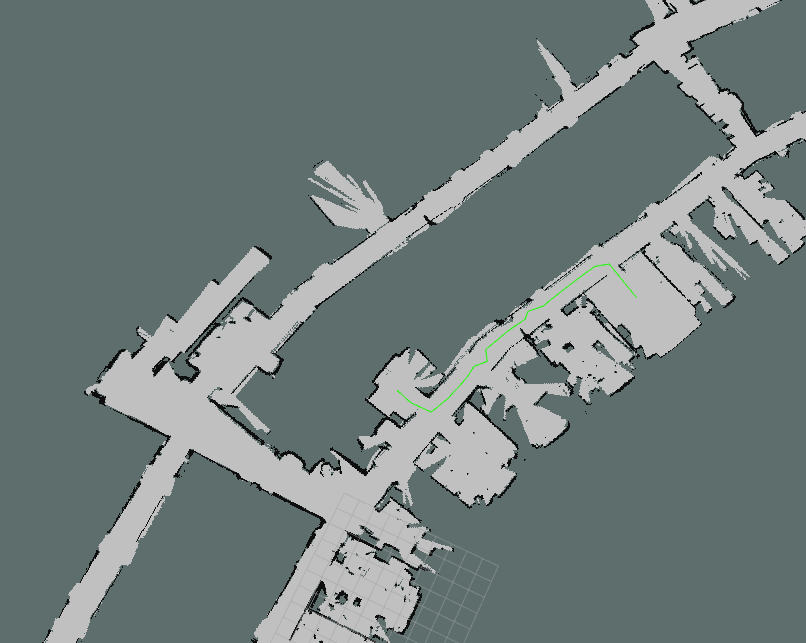
\includegraphics[width=0.6\linewidth]{img/Dstar_plan_ufficio_ripostiglio.png}
	\captionof{figure}{results obtained by the Dstar planner}
\end{figure}
\\
In the end, the logic transformation between the move\_base logic from ROS 1 to the Planner Server used in ROS 2 for the global planner are based on the implementation of the state machine Lyfecycle and the application of more advanced functionality of the languages used for programming.
\section{RoverRobotics Mini navigation result}
This are some images that display the Mini during navigation:\\
\begin{figure}[h]
\centering
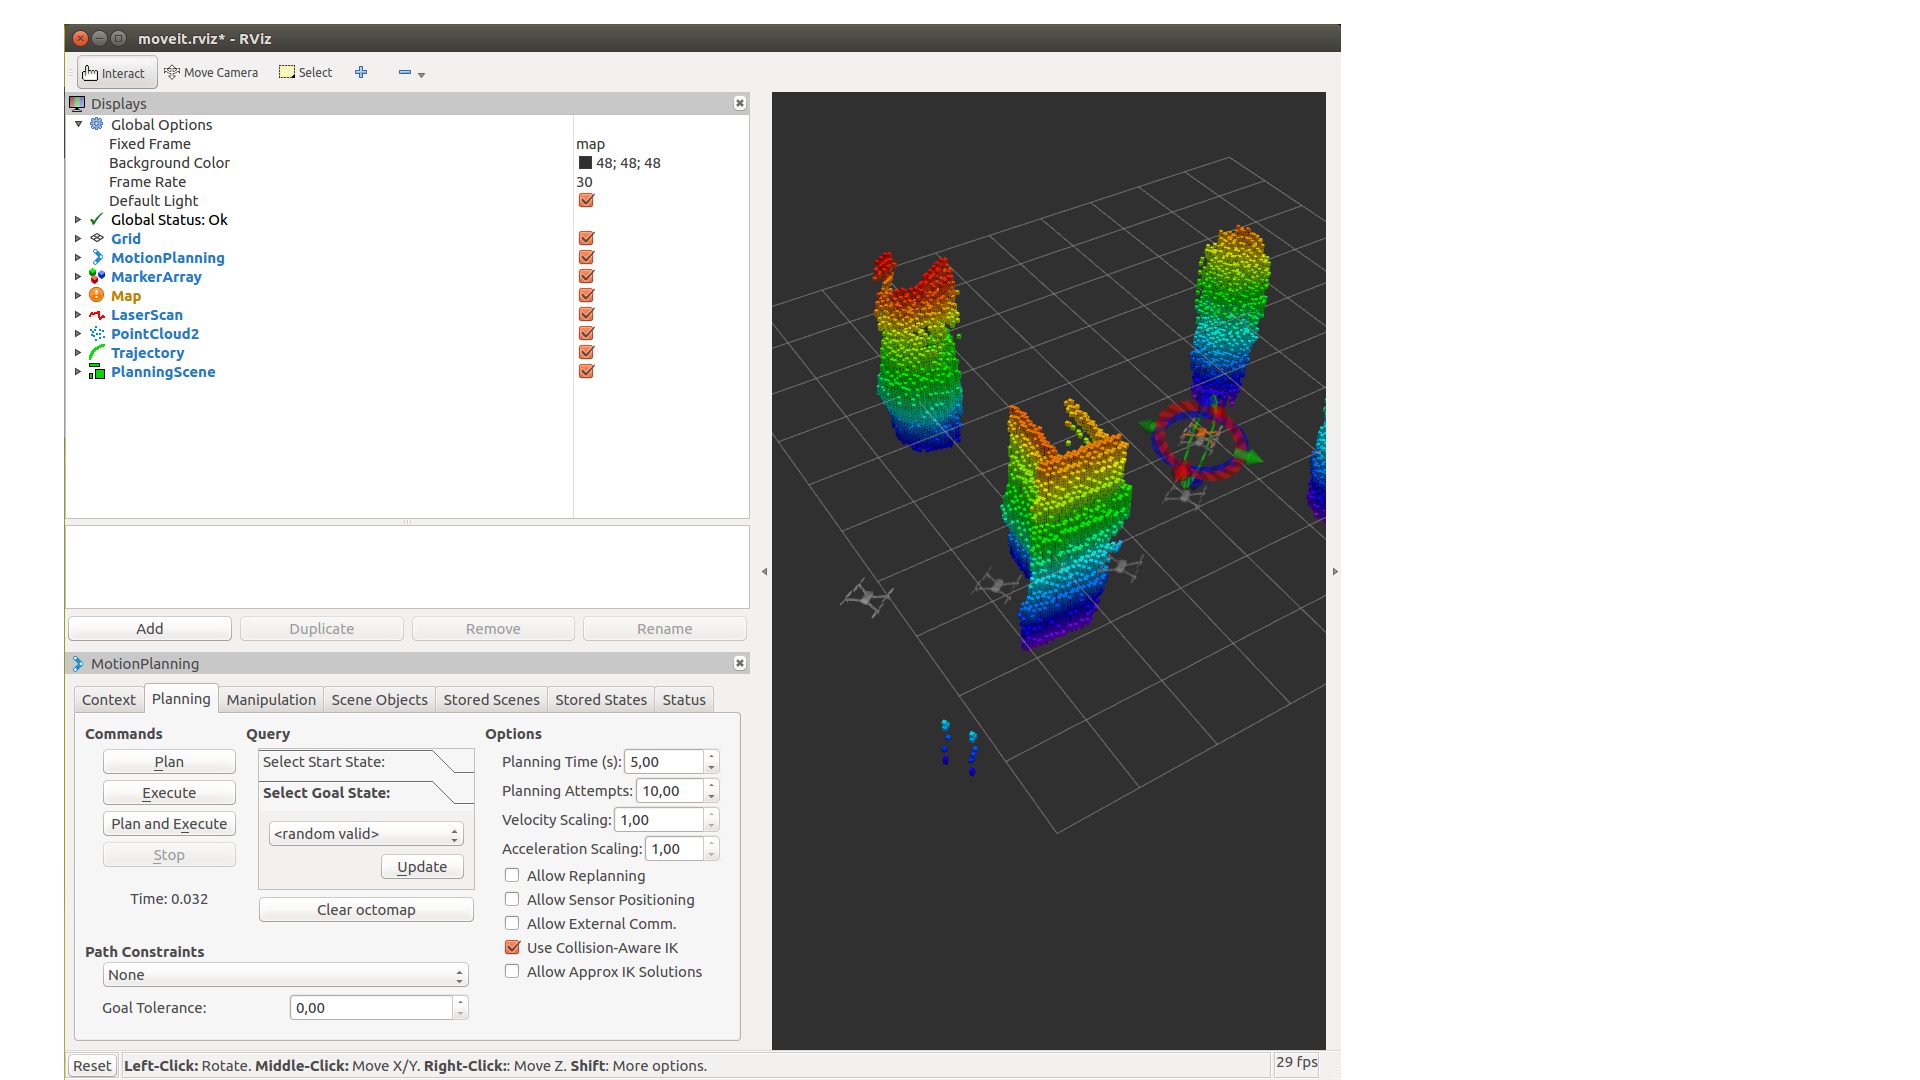
\includegraphics[width=0.7\linewidth]{img/rviz.png}
\captionof{figure}{results navigation of Mini}
\end{figure}
\\
The implementation was enough stray forward, building the robot and then apply the corrected nodes allow as to build a AMR. The tuning of the localization node and the localization node takes some time but is was reduced with the use of rosbag. 
\section{Jobot navigation result}
This are some images that display the Jobot during navigation:\\
\begin{figure}[h]
\centering
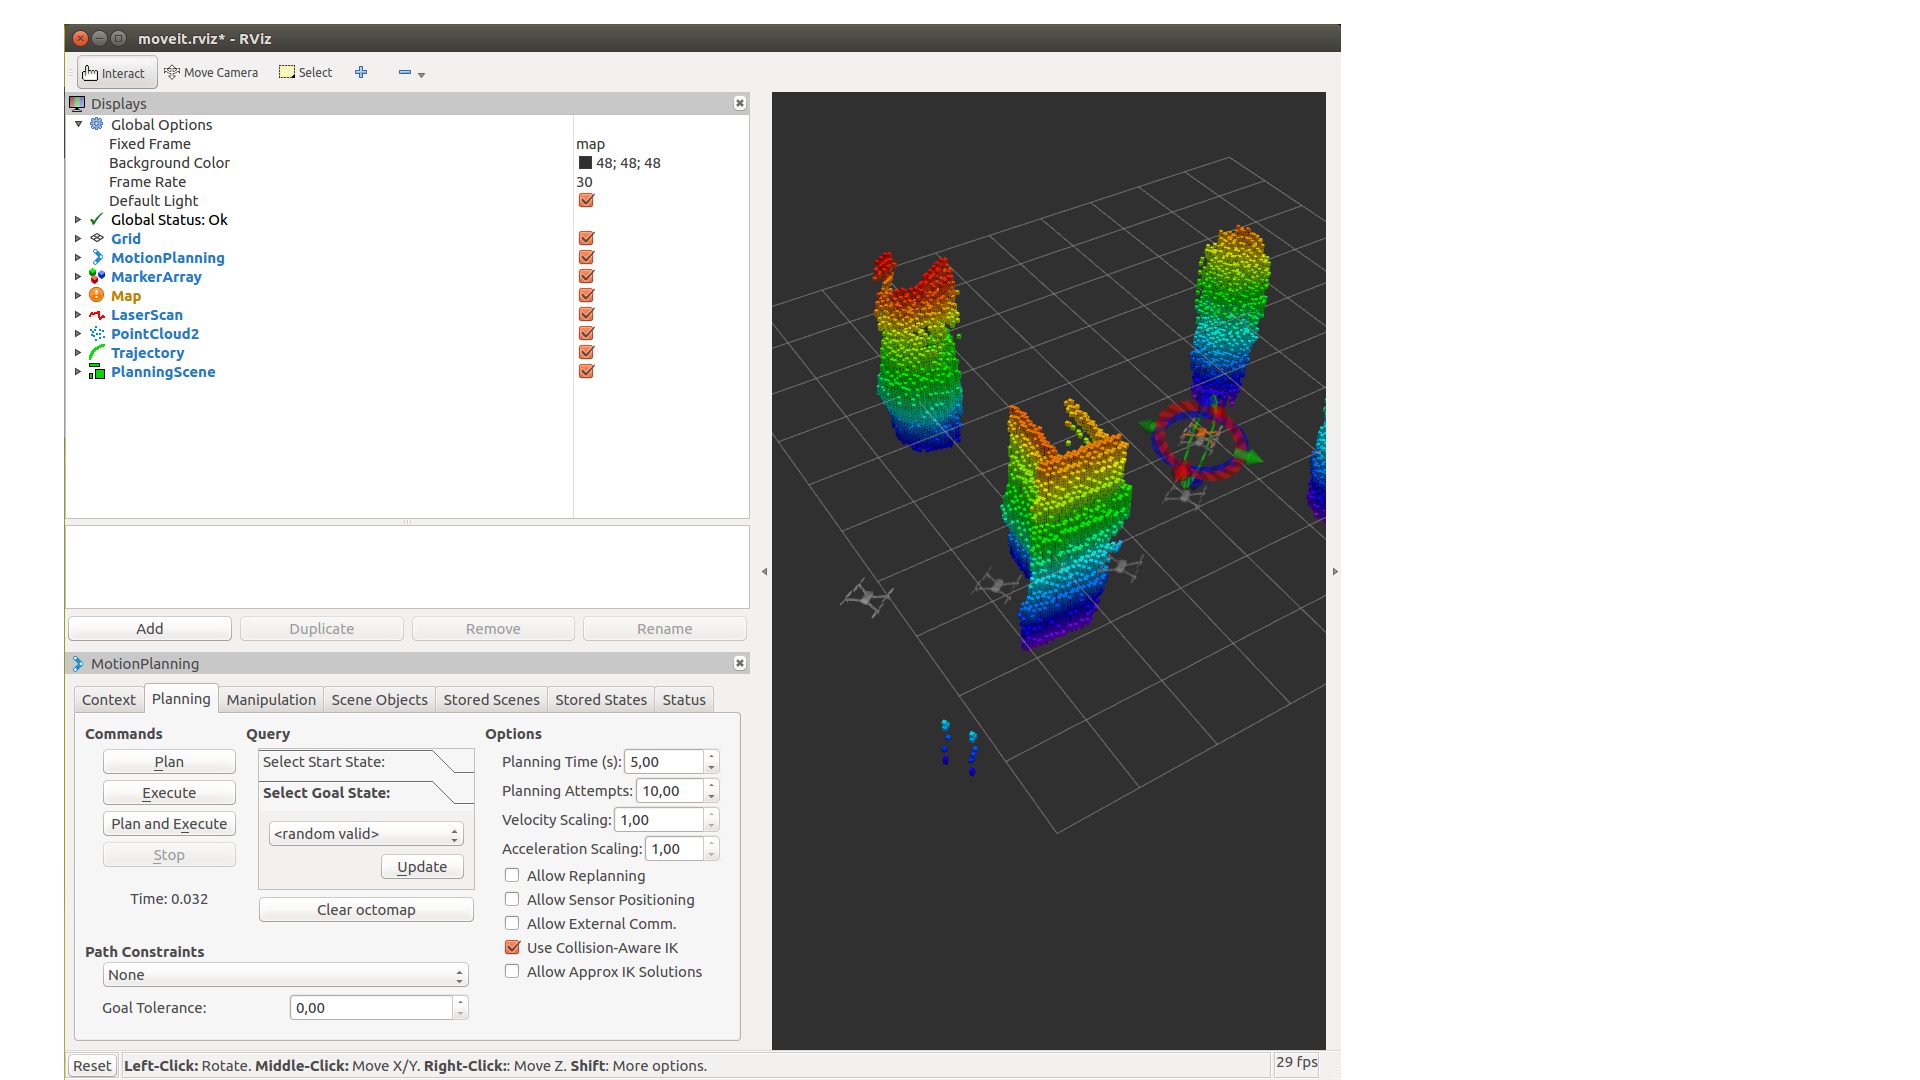
\includegraphics[width=0.7\linewidth]{img/rviz.png}
\captionof{figure}{results navigation of jobot}
\end{figure}
\\
Similar to the Mini, just more tuning.
\section{Open-RMF navigation result}
These are some images of the navigation of the 2 robots\\
\begin{figure}[h]
\centering
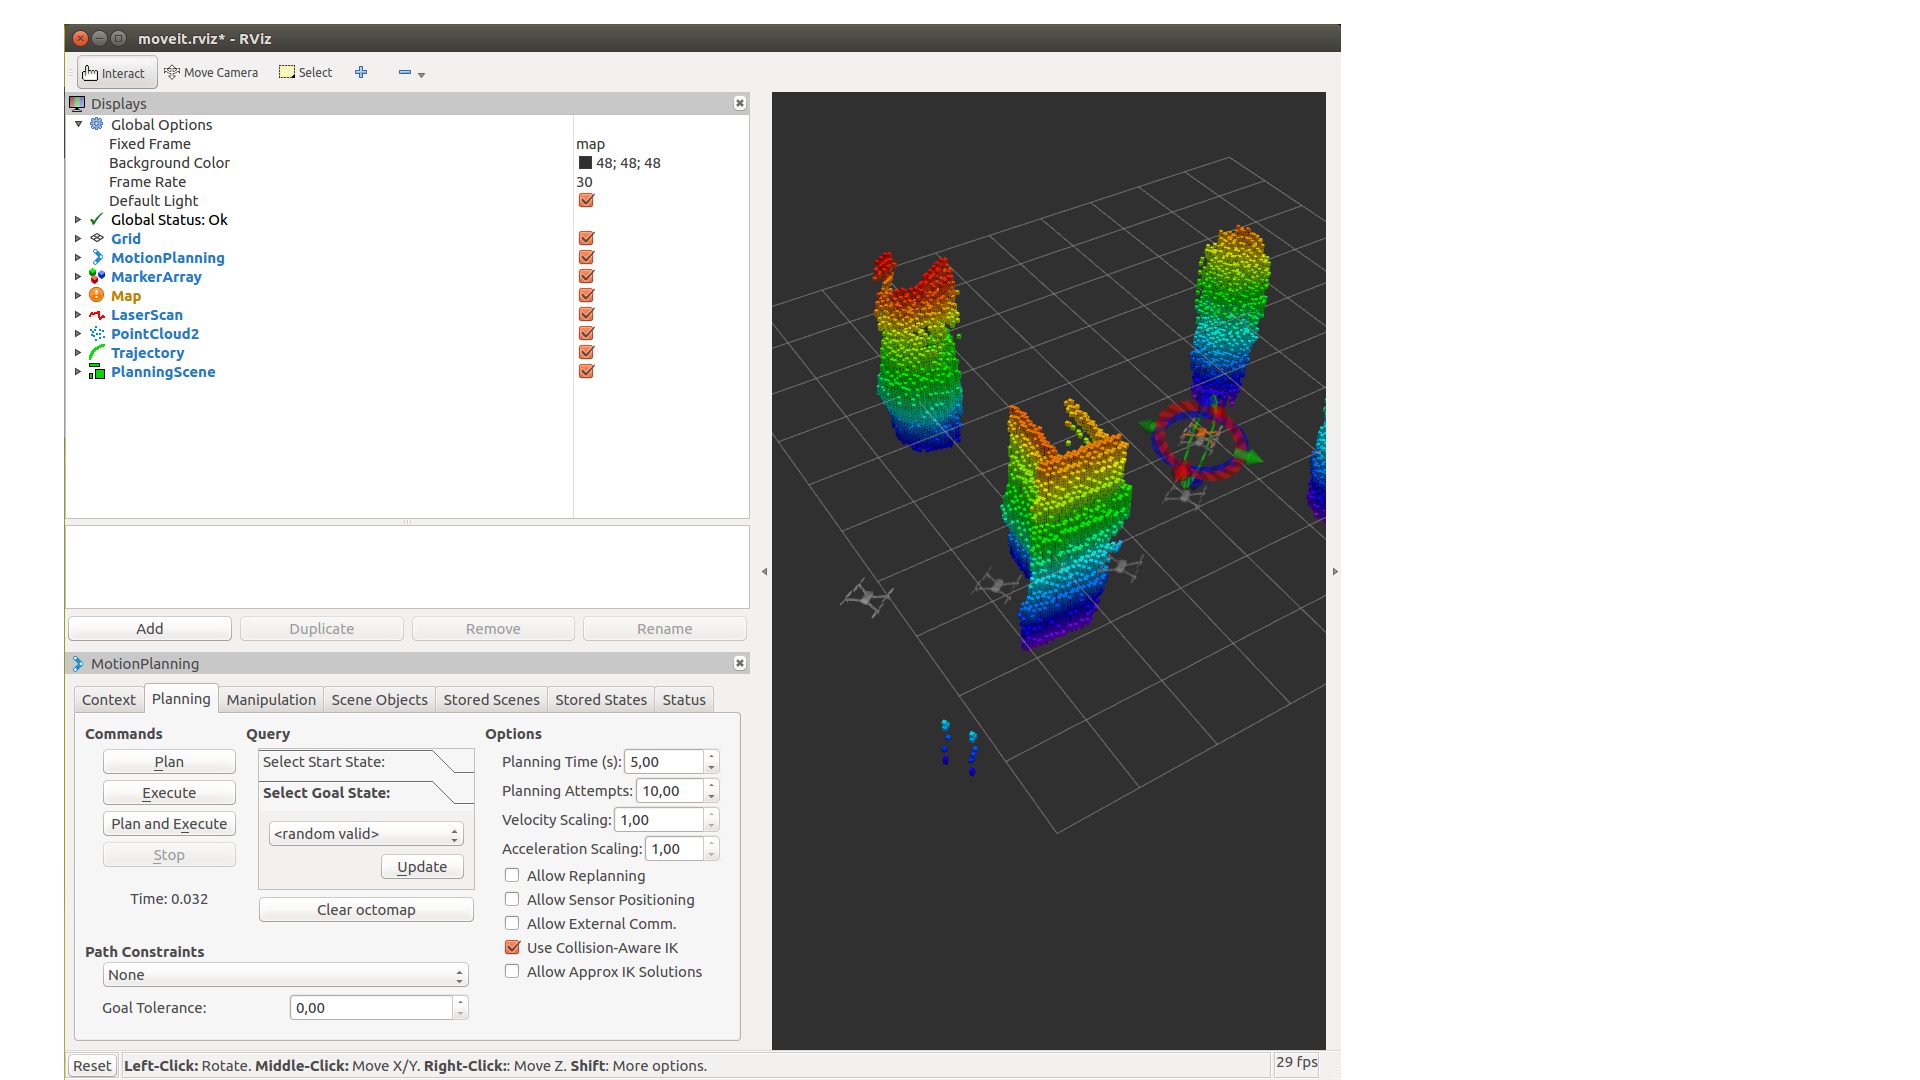
\includegraphics[width=0.7\linewidth]{img/rviz.png}
\captionof{figure}{images navigation of the 2 robots with open-rmf}
\end{figure}\\

\chapter{Comparison of system performance before and after the porting process}
This part is divided in section, in each section we evaluates the following:
\begin{itemize}
	\item calculation time for the planner on Mini rover
	\item navigation response from ROS 1 to ROS 2
\end{itemize}

\section{Planner calculation time comparisation before and after and vs new nav2 planner}
In this section, we present the time required for the global planner node to calculate the path from the planners, comparing the performance between the Jobot robot with ROS 1 built-in and the Docker ROS 2 image using the standard planner. \\
\begin{table}[h]
	\centering
	\begin{tabular}{|c|c|c|c|}
		\hline
		Start->End & ROS 1 D-start & ROS 2 D-start & ROS 2 NavfnPlanner \\
		\hline
		ufficio -> magazzino & 16.86 & 1.35 & 0.046 \\
		\hline
		ufficio -> ingresso & 73.238 & 1.35 & 0.073 \\
		\hline
		ingresso -> disegnatori & 60.41 & 1.35 & 0.081 \\
		\hline
	\end{tabular}
	\caption{result planner first request}
\end{table}\\
After the first iteration:
\begin{table}[h]
	\centering
	\begin{tabular}{|c|c|c|c|}
		\hline
		Start->End & ROS 1 D-start & ROS 2 D-start & ROS 2 NavfnPlanner \\
		\hline
		ufficio -> magazzino & 0.025 & 1.35 & 0.052 \\
		\hline
		ufficio -> ingresso & 0.091 & 1.35 & 0.069 \\
		\hline
		ingresso -> disegnatori & 0.158 & 1.35 & 0.084 \\
		\hline
	\end{tabular}
	\caption{result planner first request}
\end{table}\\

these are some results generated using the planner Dstar\\

\begin{figure}[h]
	\begin{subfigure}{.5\textwidth}
		\centering
		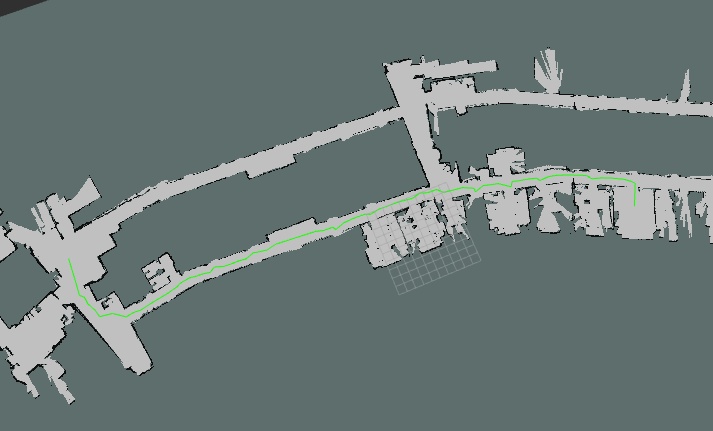
\includegraphics[width=.8\linewidth]{img/Dstar_plan_ufficio_ingresso.png}
	\end{subfigure}%
	\begin{subfigure}{.5\textwidth}
		\centering
		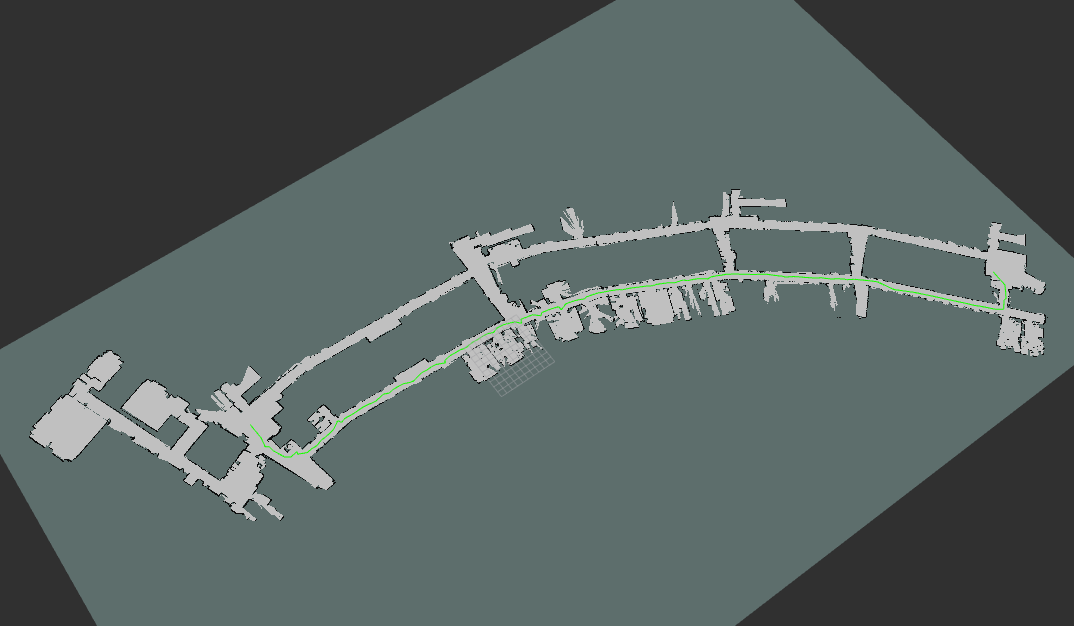
\includegraphics[width=.8\linewidth]{img/Dstar_plan_disegnatori_ingresso.png}
	\end{subfigure}
	\captionof{figure}{some of the plan generated by Dstar planner}
\end{figure}

and these are some generated by the NavfnPlanner

\begin{figure}[h]
	\begin{subfigure}{.5\textwidth}
		\centering
		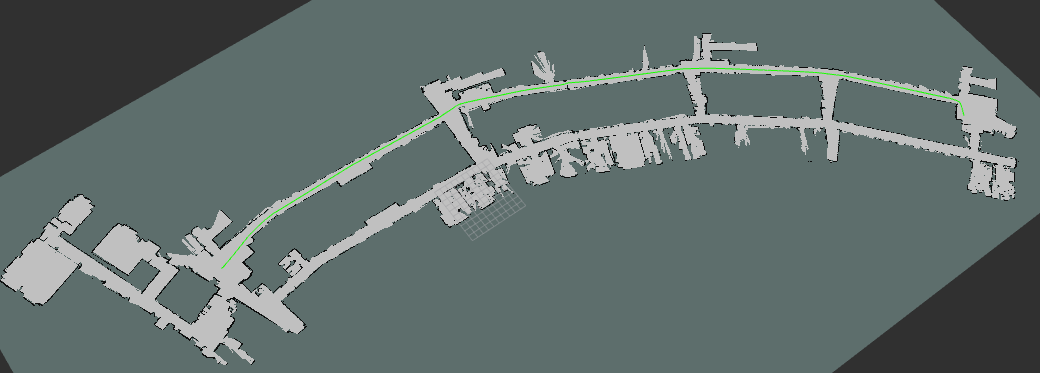
\includegraphics[width=.8\linewidth]{img/Navfn_plan_disegnatori_ingresso.png}
	\end{subfigure}%
	\begin{subfigure}{.5\textwidth}
		\centering
		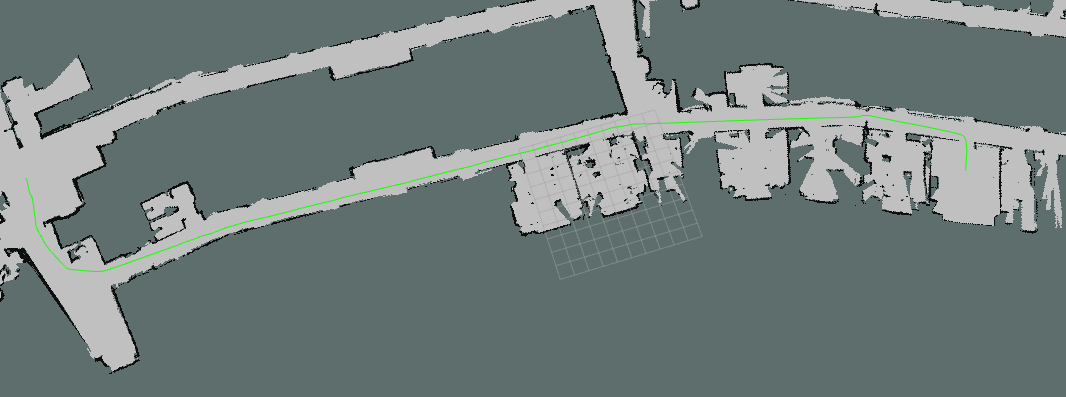
\includegraphics[width=.8\linewidth]{img/Navfn_plan_ufficio_ingresso.png}
	\end{subfigure}
	\captionof{figure}{some of the plan generated by NavfnPlanner planner}
\end{figure}

the result showed us:
\begin{itemize}
	\item time to calculate the first plan using Dstar is very higher than the NavfnPlanner
	\item after the first calculation the performances are similar
	\item without a fine tuning of the parameters of the Dstar planner hasnt returned an sub-optimal path
\end{itemize}

while porting there are some advantages that suggested an sub optimal application for open-rmf. it has an implemented a load from a file of paths but these need to reverse ingegneer to wrote down a json file compatible with that. A solution is to implement in the code a saving option for the planner.
 

\section{comparisation jobot navigation}
the test are performed using the same points as used before
\begin{table}[h]
	\centering
	\begin{tabular}{|c|c|c|}
		\hline
		Start->End & ROS 1 D-start & ROS 2 D-start \\
		\hline
		ufficio -> magazzino & 1.25 & 1.35\\
		\hline
		ufficio -> pausa lontana 1 & 1.25 & 1.35\\
		\hline
		magazzino -> pausa lontana 2 & 1.25 & 1.35\\
		\hline
	\end{tabular}
	\caption{result planner asking the node}
\end{table}
we obtain the following conclusion

\section{result analysis from Open-RMF}

\chapter{Discussion on the challenges encountered and how they were addressed}
the chalenges are:
\begin{itemize}
	\item high error on localization moving forward, it over estimate the movement comparing the map
	\item communication throught the wifi, since that the 
\end{itemize}



